\begin{appendix}

\chapter{}

\section{Compact Packings}
\label{sec:compact}

A compact packing is an arrangement of disks such that for each neighbour $D_i$ of a central disk $D$, there exists two discs $D_{i+1}$ and $D_{i-1}$ neighbour both $D_i$ and $D$~\cite{heppes:03,kennedy:06}. These packings are the most efficient way to pack space. There are a number of binary compact packings~\figref{compact packing} suitable for patterning with molecules.
\begin{figure}[htb]
    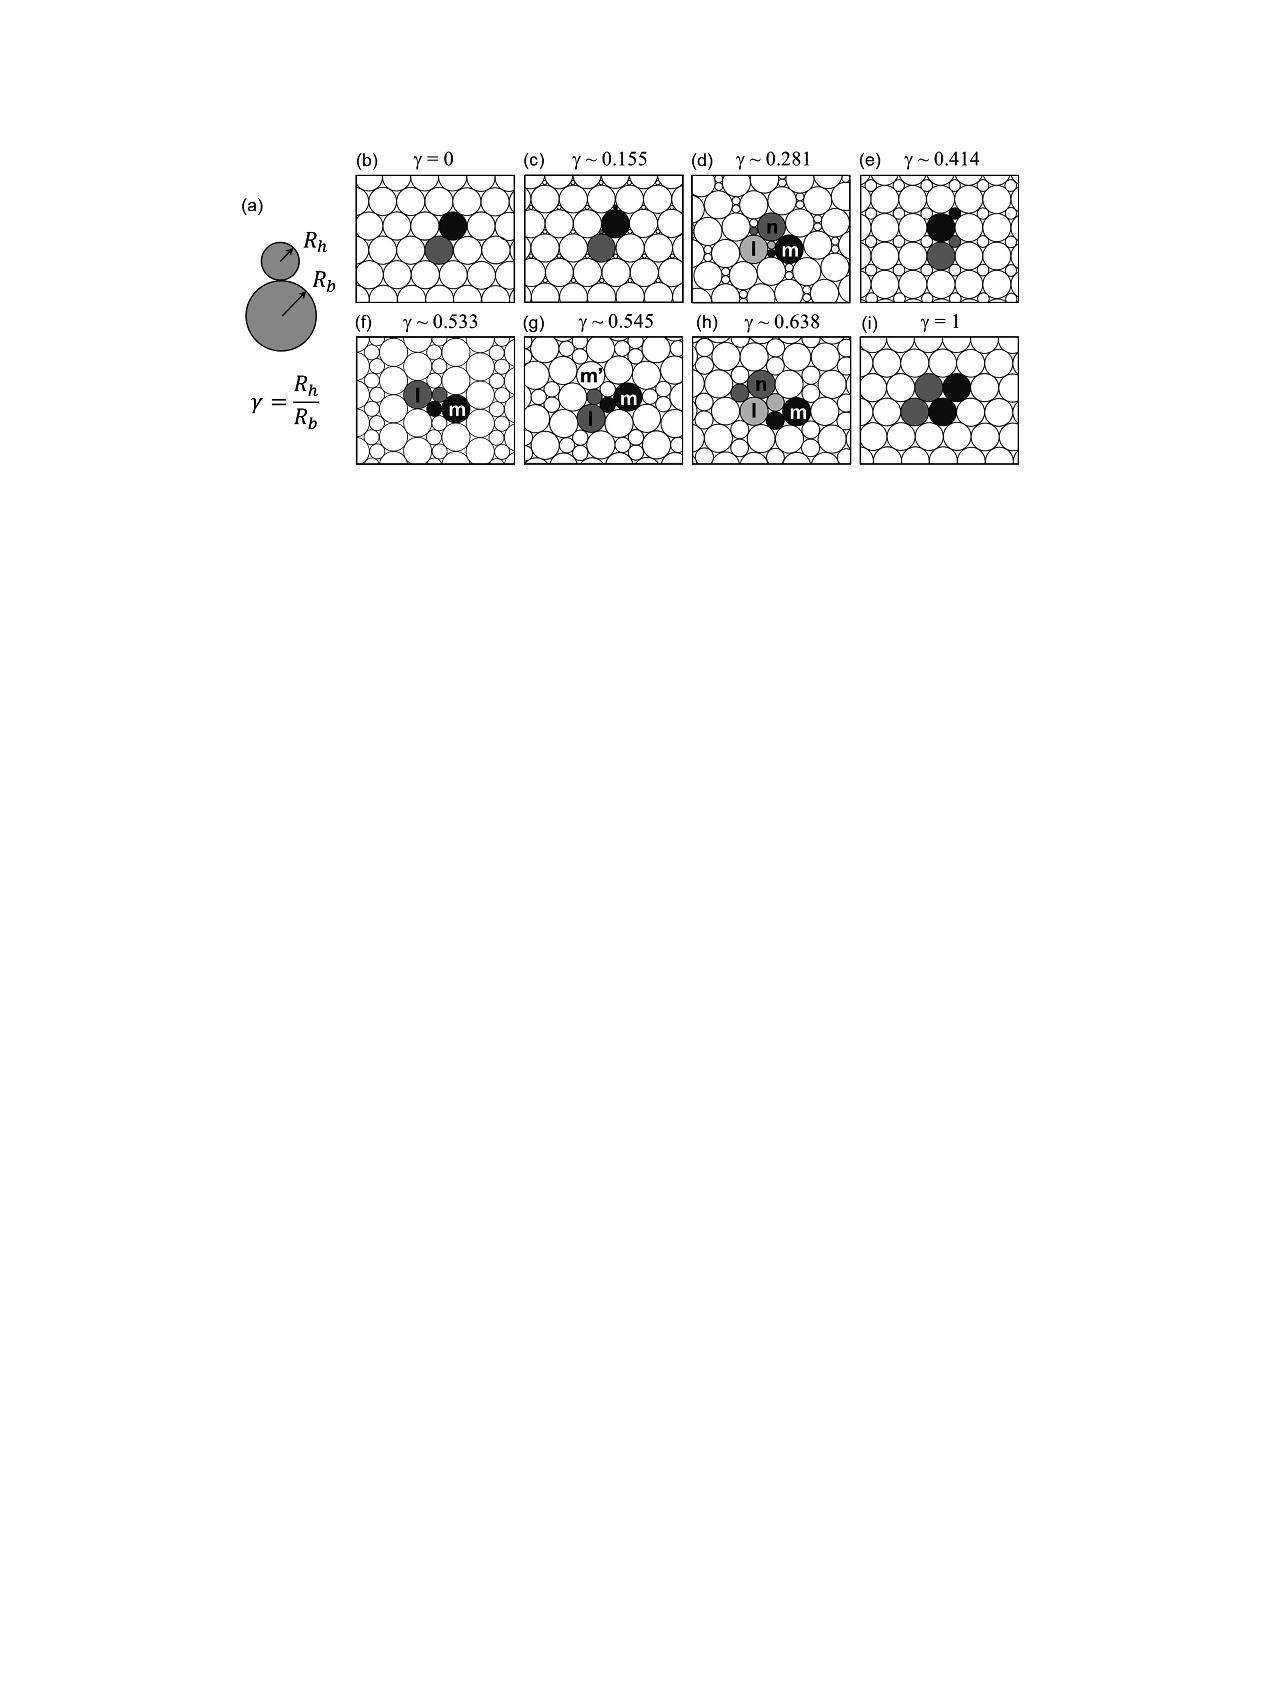
\includegraphics[width=\textwidth]{compact-packing}
    \caption{All the binary compact packings and allocations of molecules. The packing we are using in this thesis is (h).}
    \source{han:13}{American Physical Society}
    \label{fig:compact packing}
\end{figure}

\vspace{-3em}
\section{Wallpaper Groups}
\label{sec:wallpaper}

Wallpaper groups are a series of symmetry operations; rotations, mirror planes, and glide planes that describe the symmetry of a unit cell. There are 17 wallpaper groups in all and the low rotational symmetry wallpaper groups, including all wallpaper groups mentioned in this thesis are shown in \textfigref{wallpaper}
\begin{figure}[hbt]
    \centering
    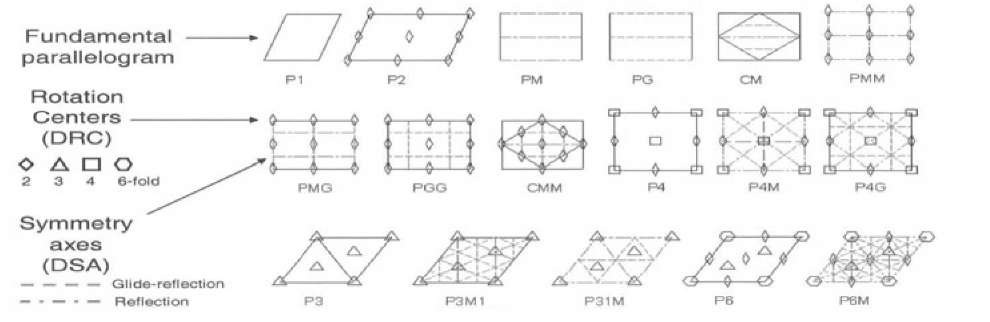
\includegraphics[width=\textwidth]{wallpaper_groups}
    \caption{The low rotational symmetry wallpaper groups showing the symmetry elements that comprise them.}
    \source[ccpd]{gagern:08}
    \label{fig:wallpaper}
\end{figure}
\end{appendix}
